%\tikzsetnextfilename{waveguidefig2} % name for the temporary 
\definecolor{cbebebf}{RGB}{200,200,200}%
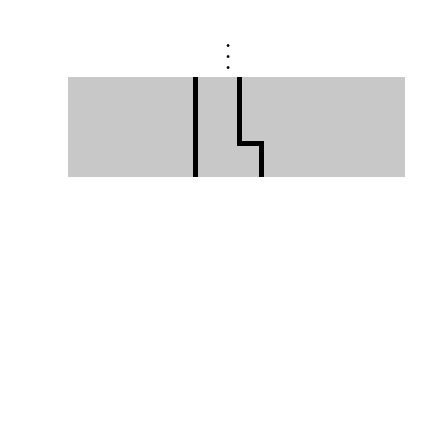
\begin{tikzpicture}[remember picture, y=0.80pt,x=0.80pt,yscale=-0.25,xscale=0.25, inner sep=0pt, outer sep=0pt]
  %\path [use as bounding box,red] (300,112) rectangle (20.0000,292.36);
  \path[fill=cbebebf,line join=miter,line cap=butt,even odd rule,line
    width=0.800pt,rounded corners=0.0000cm] (70.0000,112.3622) rectangle
    (680.0000,292.3622);
  \node at (360,60) {$\vdots$};
  \node at (0.0000,180) (myref) {};
%  \path[draw=black,line join=miter,line cap=butt,line width=0.800pt]
%    (650.0000,112.3622) .. controls (100.0000,112.3622) and (100.0000,112.3622) ..
%    (100.0000,112.3622);
%  \path[draw=black,line join=miter,line cap=butt,line width=0.800pt]
%    (650.5000,291.8622) .. controls (100.5000,291.8622) and (100.5000,291.8622) ..
%    (100.5000,291.8622);
  \path[draw=black,line join=miter,line cap=butt,line width=1.800pt]
    (300.0000,112.3622) -- (300.0000,292.3622) -- (300.0000,292.3622);
  \path[draw=black,line join=miter,line cap=butt,line width=1.800pt]
    (380.0000,112.3622) -- (380.0000,232.3622) -- (420.0000,232.3622) --
    (420.0000,292.3622) -- (420.0000,292.3622);
  \path[fill=black] (255.56859,334.04221) node (text3878) {\phantom{$\;\;\;\partial\Omega_-$}};
  \path[fill=black] (440.42651,334.04221) node[right] (text3882) {\phantom{$\partial\Omega_+$   }};
  \node at (0,690) {};
\end{tikzpicture}%
\begin{tikzpicture}[remember picture, y=0.80pt,x=0.80pt,yscale=-0.25,overlay, shift={(myref.north)}, xscale=0.25, inner sep=0pt, outer sep=0pt]
  \path[fill=cbebebf,line join=miter,line cap=butt,even odd rule,line
    width=0.800pt,rounded corners=0.0000cm] (70.0000,112.3622) rectangle
    (680.0000,292.3622);
  \node at (0.0000,180) (myref2) {};
%  \path[draw=black,line join=miter,line cap=butt,line width=0.800pt]
%    (650.0000,112.3622) .. controls (100.0000,112.3622) and (100.0000,112.3622) ..
%    (100.0000,112.3622);
%  \path[draw=black,line join=miter,line cap=butt,line width=0.800pt]
%    (650.5000,291.8622) .. controls (100.5000,291.8622) and (100.5000,291.8622) ..
%    (100.5000,291.8622);
  \path[draw=black,line join=miter,line cap=butt,line width=1.800pt]
   (300.0000,112.3622) -- (300.0000,292.3622) -- (300.0000,292.3622);
  \path[draw=black,line join=miter,line cap=butt,line width=1.800pt]
    (425,112.3622) --  (380.0000,112.3622) -- (380.0000,232.3622) -- (420.0000,232.3622) --
    (420.0000,292.3622) -- (420.0000,292.3622);
\end{tikzpicture}%
\begin{tikzpicture}[remember picture, y=0.80pt,x=0.80pt,yscale=-0.25,overlay, shift={(myref2.north)}, xscale=0.25, inner sep=0pt, outer sep=0pt]
  \path[fill=cbebebf,line join=miter,line cap=butt,even odd rule,line
    width=0.800pt,rounded corners=0.0000cm] (70.0000,112.3622) rectangle
    (680.0000,292.3622);
  \node at (0.0000,180) (myref3) {};
%  \path[draw=black,line join=miter,line cap=butt,line width=0.800pt]
%    (650.0000,112.3622) .. controls (100.0000,112.3622) and (100.0000,112.3622) ..
%    (100.0000,112.3622);
%  \path[draw=black,line join=miter,line cap=butt,line width=0.800pt]
%    (650.5000,291.8622) .. controls (100.5000,291.8622) and (100.5000,291.8622) ..
%    (100.5000,291.8622);
  \path[draw=black,line join=miter,line cap=butt,line width=1.800pt]
   (300.0000,112.3622) -- (300.0000,292.3622) -- (300.0000,292.3622);
  \path[draw=black,line join=miter,line cap=butt,line width=1.800pt]
    (425,112.3622) --  (380.0000,112.3622) -- (380.0000,232.3622) -- (420.0000,232.3622) --
    (420.0000,292.3622) -- (420.0000,292.3622);
  \path[<->,draw=black,line width=1pt]
    (100.0000,150) -- node[midway,left] {$z$\;\;} (100.0000,240) -- node[midway,below]{$\phantom{\Sigma^\Sigma}x\phantom{\Sigma^\Sigma}$} (200,240);
  \node at (360,320) {$\vdots$};
\end{tikzpicture}%
